% Feel free to contact me for any reason:
%% Email 1: zain.kamal@rutgers.edu
%% Email 2: z.kamal2021@gmail.com
%% Discord: alci#6038

%%%%%%%%%%%%%%%%%%%%%%%%%%%%%%%%%%%%%%%%%%%%%%%%%%%%%%%%%%%%%%%%%%%%%%%%%%%%%%%%%
\documentclass{article}
% Feel free to contact me for any reason:
%% Email 1: zain.kamal@rutgers.edu
%% Email 2: z.kamal2021@gmail.com
%% Discord: alci#6038

% Last updated 1/28/22

% Template based off of Justin Kim's (don't know where he got it from originally), but I've made a ton of edits. His soul lives on in random packages and commands I'm too lazy to comment out.


%%%%%%%%%%%%%%%%%%%%%%%%%%%%%%%%%%%%%%%%%%%%%%%%%%%%%%%%%%%%%%%%%%%%%%%%%%%%%%%%%%%%
%%% Default packages:

\usepackage[margin=1in]{geometry} 
\usepackage{amsmath,amsthm,amssymb,amsfonts, fancyhdr, color, comment, graphicx, environ}
\usepackage{xcolor}
\usepackage{mdframed}
\usepackage{bm}
\usepackage[shortlabels]{enumitem}
\usepackage{mathtools}
\usepackage{listings}
\usepackage{stmaryrd}
\usepackage{indentfirst}
\usepackage{hyperref}


%%%%%%%%%%%%%%%%%%%%%%%%%%%%%%%%%%%%%%%%%
%%% Pacakages I've added:

%% For Math 300 (Winter 2021):

\usepackage{mathdots} % for \iddots

\usepackage[ruled]{algorithm2e} % Algorithms
% NOTE: FIND A BETTER ALGORITHM PACKAGE, OR ATLEAST LEARN HOW TO USE THIS ONE BECAUSE DOUBLE INDENTING IS A FUCKING NIGHTMARE (or just import from mathcha?)
%% Example algorithm:
% \begin{center}
% 	\begin{minipage}{0.5\linewidth} % Adjust the minipage width to accomodate for the length of algorithm lines
% 		\begin{algorithm}[H]
% 			\KwIn{$(a, b)$, two floating-point numbers}  % Algorithm inputs
% 			\KwResult{$(c, d)$, such that $a+b = c + d$} % Algorithm outputs/results
% 			\medskip
% 			\If{$\vert b\vert > \vert a\vert$}{
% 				exchange $a$ and $b$ \;
% 			}
% 			$c \leftarrow a + b$ \;
% 			$z \leftarrow c - a$ \;
% 			$d \leftarrow b - z$ \;
% 			{\bf return} $(c,d)$ \;
% 			\caption{\texttt{FastTwoSum}} % Algorithm name
% 			\label{alg:fastTwoSum}   % optional label to refer to
% 		\end{algorithm}
% 	\end{minipage}
% \end{center}



%%%%%%%%%%%%%%%%%%%%%%%%%%%%%%%%%%%%%%%%%%%%%%%%%%%%%%%%%%%%%%%%%%%%%%%%%%%%%%%%%%%%
%%% Default commands:

\renewcommand{\vec}[1]{\mathbf{#1}}
	
\newcommand{\WidestEntry}{$lon_1$}%
\newcommand{\SetToWidest}[1]{\makebox[\widthof{\WidestEntry}]{#1}}%
\newcommand\tab[1][0.61cm]{\hspace*{#1}}
\newcommand{\nats}{\mathbb{N}}
\newcommand{\rats}{\mathbb{Q}}
\newcommand{\reals}{\mathbb{R}}
\newcommand{\Z}[1]{\mathbb{Z}_{#1}}
\newcommand{\BigO}[1]{\mathcal{O}(#1)}
\newcommand{\seq[1]}{(#1_n)}
\newcommand{\subseq[1]}{(#1_{n_k})}
\newcommand{\Lim}[2]{\lim \limits _{#1 \to #2}}
\newcommand{\Min}[2]{\min \{#1, #2\}}
\newcommand{\inv}{^{-1}}
\newcommand{\h}{^\text{th}}
\newcommand{\lrangle}[1]{\langle #1 \rangle}
\newcommand{\abs}[1]{\left\lvert #1 \right\rvert}

\DeclarePairedDelimiter{\ceil}{\lceil}{\rceil}
\DeclarePairedDelimiter{\floor}{\lfloor}{\rfloor}
\DeclareMathOperator{\supp}{supp}
\DeclareMathOperator{\rad}{rad}
\DeclareMathOperator*{\argmin}{arg\,min}
\DeclareMathOperator*{\argmax}{arg\,max}
\DeclareMathOperator*{\Var}{Var}
\DeclareMathOperator*{\Cov}{Cov}
\DeclareMathOperator*{\Corr}{Corr}
\DeclareMathOperator*{\Aut}{Aut}
\newcommand{\prob}[1]{\section*{Problem #1}}


%%%%%%%%%%%%%%%%%%%%%%%%%%%%%%%%%%%%%%%%%
%%% Commands I've added:

%% For Math 300 (Winter 2021):

\newcommand{\lrbrace}[1]{\{ #1 \}}
\newcommand{\powerset}{\mathcal{P}}
\newcommand{\ints}{\mathbb{Z}}

% Source/inspiration: https://tex.stackexchange.com/a/42728:
\newcommand{\numberthis}{\addtocounter{equation}{1}\tag{\theequation}\label{\theequation}}
    % Within an `align*` environment, put `\numberthis` after a line to number it. 
    % Access it with `\eqref{ [number of equation] }`
\newcommand{\numberthiswith}[1]{\addtocounter{equation}{1}\tag{\theequation}\label{#1}}
    % Within an `align*` environment, put `\numberthiswith{ [your_label] }` after a line to number it. 
    % Access it with `\eqref{ [your_label] }`



%%%%%%%%%%%%%%%%%%%%%%%%%%%%%%%%%%%%%%%%%%%%%%%%%%%%%%%%%%%%%%%%%%%%%%%%%%%%%%%%%%%%
%%% Default formatting:

\hypersetup{
    colorlinks=true,
    linkcolor=blue,
    filecolor=magenta,      
    urlcolor=blue,
}

\setlength{\parindent}{0cm}
\setlength{\parskip}{6pt}

\pagestyle{fancy}


%% Misc formatting additions

% make bullets with itemize much smaller
\newlength{\mylen}
\setbox1=\hbox{$\bullet$}\setbox2=\hbox{\tiny$\bullet$}
\setlength{\mylen}{\dimexpr0.5\ht1-0.5\ht2}
\renewcommand\labelitemi{\raisebox{\mylen}{\tiny$\bullet$}}


% Modified version of problem environment below
% \newenvironment{problem}[2][Problem]
%     { \begin{mdframed}[backgroundcolor=gray!5] \textbf{#1 #2} \\}
%     {  \end{mdframed}}
% \newenvironment{solution}{\textbf{Solution}\\}


%%%%%%%%%%%%%%%%%%%%%%%%%%%%%%%%%%%%%%%%%
%%% Formatting I've added:

%% Grey boxes for problem statements (note that I don't have a "solution" section):

% Problem environment, but shows "(a)" instead of "Problem a"
\newenvironment{problem}[2][]
    { \begin{mdframed}[backgroundcolor=gray!5] \textbf{#1 (#2)}}
    {  \end{mdframed}}
% Problem environment, but no "([input_char])" at all
\newenvironment{problem*}
    { \begin{mdframed}[backgroundcolor=gray!5] \\}
    {  \end{mdframed}}


% Example environment, currently identical to "problem" (Note: this is better written than the problem environment because I wrote it myself from scratch. Use this as an example for future new environments.)
\newcounter{example}[section]
\newenvironment{example}
    { 
        \refstepcounter{example}
        \begin{mdframed}[backgroundcolor=gray!5]
        \textbf{\\Example \thesection.\theexample:}
    }
    {\\ \end{mdframed}}


%%%%%%%%%%%%%%%%%%%%%%%%%%%%%%%%%%%%%%%%%%%%%%%%%%%%%%%%%%%%%%%%%%%%%%%%%%%%%%%%%%%%
% Misc things I've added




%%%%%%%%%%%%%%%%%%%%%%%%%%%%%%%%%%%%%%%%%%%%%
% Fill in the appropriate information below
\lhead{Zain Kamal}
% \rhead{Math 244 Spring 2022} % Moved to document
% \chead{\textbf{Homework 2}} % Moved to document
\begin{document}
\chead{\textbf{Physics 351: Homework 1}}
\rhead{2/3/22}
%%%%%%%%%%%%%%%%%%%%%%%%%%%%%%%%%%%%%%%%%%%%%%%%%%%%%%%%%%%%%%%%%%%%%%%%%%%%%%%%%

\textbf{\underline{1.10}}
\begin{align*}
PV & =NkT\\
( 1\ atm)( 4\ m)^{3} & =N\left( 0.082057\ \frac{L\cdot atm}{mol\cdot K}\right)( 293\ K)\\
\Rightarrow N & =2.66\ mol
\end{align*}
\

\hline

\textbf{\underline{1.13}}



$H_{2} O:$ $16+2+2=18$ g/mol



$N_{2} :14\cdot 2=18$ g/mol



$Pb:207$ g/mol



$SiO_{2} :28+16\cdot 2=60$ g/mol



\

\hline

\textbf{\underline{1.16}}

(a)

Let pressure be a function of $z$:

\begin{figure}[htp]
    \centering
    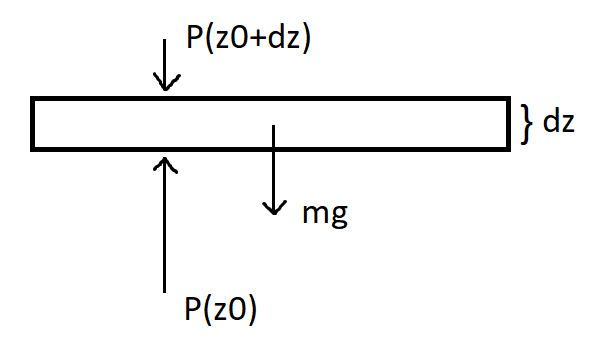
\includegraphics[width=12cm]{images/weh.png}
\end{figure}

Considering the free-diagram of a slab of air at rest, we can find:
\begin{align*}
P( z_{0} +dz) \cdot A+mg & =P( z_{0}) \cdot A\\
P( z_{0} +dz) -P( z_{0}) & =-\frac{mg}{A}\\
dP & =-\frac{mg}{A} .
\end{align*}
Let the density of the slab of air be given by $\rho =\frac{m}{V}$. Then:
\begin{align*}
dP & =-\frac{\rho Vg}{A} .
\end{align*}
Since $V$ and $A$ both describe the dimensions of the slab of air, dividing them gives us the height of the slab, $dz$:
\begin{align*}
\frac{dP}{dz} & =-\rho g.
\end{align*}


\

(b)

Let $m$ be the molar mass of a molecule. Then we can find the mass $M$:
\begin{align*}
PV & =NkT\\
PV & =\left(\frac{M}{m}\right) kT\\
\Rightarrow m & =\frac{MkT}{PV} .
\end{align*}
We can then calculate density:
\begin{align*}
\rho  & =\frac{m}{V}\\
 & =\frac{mP}{kT} .
\end{align*}
Substititing this into the differential equation from (a) yields:
\begin{align*}
\frac{dP}{dz} & =-\frac{mgP}{kT} .
\end{align*}


\

(c)

We solve:
\begin{align*}
\frac{dP}{dz} & =-\frac{mgP}{kT}\\
\int \frac{dP}{P} & =\int -\frac{mg}{kT} \ dz\\
\ln |P| & =\frac{-mgz}{kT}\\
\Rightarrow P( z) & =e^{\frac{-mgz}{kT}} .
\end{align*}
In the above equation, we see $P( 0) =1$. So we add $P_{0}$, or the initial pressure at $z=0$:
\begin{equation*}
\boxed{P( z) =P_{0} e^{\frac{-mgz}{kT}} .}
\end{equation*}


\

\hline

\textbf{\underline{1.18}}

For all locations, let $P_{0} =1\ atm$, let the air be 80\% nitrogen and 20\% oxygen ($m=0.8\cdot ( 14.01\cdot 2) +0.2( 16.00\cdot 2) =28.816\ g/mol$), and let $T=273K$. Thus we calculate:
\begin{itemize}
\item Ogden, Utah: $P( 1430\ m) =0.84\ atm$
\item Leadville, Colorado: $P( 3090\ m) =0.69\ atm$
\item Mt. Whitney, California: $P( 4420\ m) =0.60\ atm$
\item Mt. Everest, Nepal Tibet: $P( 8840\ m) =0.35\ atm$
\end{itemize}



\

\hline

\textbf{\underline{1.21}}

We calculate the average pressure:
\begin{align*}
P & =\frac{F}{A}\\
 & =\frac{m\ \frac{dv}{dt}}{A}\\
 & =( 0.002\ kg)\frac{2\left( 15\frac{m}{s} \cdot \cos 45\ \right)}{\left(\frac{1}{30} \ s\right)\left( 0.5\ m^{2}\right)}\\
 & =\boxed{2.55\ N/m^{2}} .
\end{align*}


\

\hline

\textbf{\underline{1.22}}

(a)

Similar to the last question:
\begin{align*}
P & =\frac{m\ \Delta x}{A\ \Delta t} .
\end{align*}
For an ellastic collision $\Delta v_{x} =-2v_{x}$, which we average over $N$ molecules:
\begin{align*}
P & =\frac{m\ \left( 2\ N\overline{v_{x}}\right)}{A\ \Delta t} .
\end{align*}
This readily shows
\begin{equation*}
\boxed{\Delta t=\frac{m\ \left( 2\ N\overline{v_{x}}\right)}{PA} .}
\end{equation*}
\

(b)

We simply manipulate one of our given equations:
\begin{align*}
m\overline{v_{x}^{2}} & =kT\\
\Rightarrow \sqrt{\overline{v_{x}^{2}}} & =\sqrt{\frac{kT}{m}} .
\end{align*}
\

(c)

We solve the final equation from (a) for $N$ to show:
\begin{align*}
-\Delta N & =\frac{PA\ \Delta t}{2m\overline{v_{x}}} .
\end{align*}
We then substitute $\overline{v_{x}}$ from (b) to find:
\begin{equation*}
\begin{aligned}
-\Delta N & =\frac{PA\ \Delta t}{2m}\sqrt{\frac{m}{kT}} .
\end{aligned}
\end{equation*}
We then substitute the ideal gas law for $P$ and convert to a differential equation, and define the constant $\tau $:
\begin{equation*}
\begin{aligned}
\frac{dN}{dt} & =\left( -\frac{kTA}{2Vm}\sqrt{\frac{m}{kT}}\right) N.\\
 & =-\left(\frac{A}{2V}\sqrt{\frac{kT}{m}}\right) N\\
 & =-\frac{1}{\tau } N.
\end{aligned}
\end{equation*}
This can easily be solved to yield
\begin{equation*}
N( t) =N( 0) e^{\frac{-t}{\tau }}
\end{equation*}


\

(d)

Assuming the gas is air, which is mostly nitrogen:
\begin{align*}
\tau  & =\left(\frac{A}{2V}\sqrt{\frac{RT}{M}}\right)^{-1}\\
 & =\left(\frac{( 0.001\ m)^{2}}{2\left( 0.001\ m^{3}\right)}\sqrt{\frac{( 8.3\ J/mol)( 273\ K)}{0.028\ kg/mol}}\right)^{-1}\\
 & =7.03\ s.
\end{align*}
\

(e)
\begin{align*}
3600\ s & =\frac{2\left( 0.001m^{3}\right)}{A}\sqrt{\frac{0.028\ kg/mol}{( 8.3\ J/mol)( 273\ K)}}\\
\Rightarrow A & =1.95\times 10^{-9} \ m
\end{align*}
\

(f)

All of the air would escape in
\begin{align*}
\tau  & =\frac{2\left( 100\ m^{3}\right)}{( 1\ m)^{2}}\sqrt{\frac{0.028\ kg/mol}{( 8.3\ J/mol)( 273\ K)}}\\
 & =0.7s,
\end{align*}
so there's no way to quickly open and close the window and survive.





\

\hline

\textbf{\underline{1.23}}

Helium has three degrees of freedom (translational), so
\begin{align*}
U & =\frac{3}{2} PV\\
 & =\frac{3}{2}\left( 10^{6} \ N/m^{2}\right)\left( 10^{-3} \ m^{3}\right)\\
 & =150\ J.
\end{align*}
Air has five degrees of freedom (translational and rotational), so $U=\frac{5}{2} PV=250\ J$.



\

\hline

\textbf{\underline{1.33}}

(a) Work is negative as volume increases in step A, zero when the volume is constant in step B, and positive when volume is decreasing in step C. Net work is positive because step C has a greater average pressure than step A.

(b) $U=\frac{f}{2} PV$, so energy is increasing in steps A and B, and decreasing in step C. The net energy must be constant, as $P$ and $V$ don't experience any net change.

(c) $Q=\Delta U-W$, so heat is increasing in steps A and B, and decreasing in step C. Overall, we lose heat because of step C.



Effectively, this process takes in energy from some work and releases that energy as heat.












%%%%%%%%%%%%%%%%%%%%%%%%%%%%%%%%%%%%%%%%%%%%%%%%%%%%%%%%%%%%%%%%%%%%%%%%%%%%%%%%%
\end{document}